
\documentclass{beamer}
%\beamertemplateshadingbackground{brown!70}{yellow!10}
\mode<presentation>
{
  %\usetheme{Warsaw}
  \usecolortheme{crane}
  % or ...

%  \setbeamercovered{transparent}
  % or whatever (possibly just delete it)
}
\setbeamertemplate{navigation symbols}{}
%\setbeamertemplate{footline}[frame number]{}
\usepackage{tikz,pgfplots}
\pgfplotsset{compat=newest}
\usepackage[utf8]{inputenc}
\usetikzlibrary{patterns}
\usepackage{amssymb}
\usepackage{amsmath}
\usepackage{colortbl}
%\usepackage{multicol}
\usepackage{cancel}
\usepackage{ulem}
\usepackage{multirow}
\usepackage{relsize}
\usepackage{algorithm}
\usepackage{algorithmic}
\usepackage{forloop}% http://ctan.org/pkg/forloop
\newcounter{loopcntr}
\newcommand{\rpt}[2][1]{%
  \forloop{loopcntr}{0}{\value{loopcntr}<#1}{#2}%
}
%\pagestyle{plain}
%\input{defs2}
\def\opt{{\textsc{OPT}_k}}
\def\const{{\mathrm{const}}}
\def\nnz{{\mathrm{nnz}}}
\def\r{\sfrac{\sigma_{\w}^2}{\sigma_{\xib}^2}}
\def\rm{\sfrac{\sigma_{\xib}^2}{\sigma_{\w}^2}}
\def\cmark{\Green{\checkmark}}
\def\xmark{\Red{\large\sffamily x}}
\newcommand{\pdet}{{\mathrm{pdet}}}
\newcommand{\MSPE}[1] {{\mathrm{MSPE}\big[#1\big]}}
\newcommand{\MSE}[1] {{\mathrm{MSE}\big[#1\big]}}
\def\Poisson{{\operatorname{Poisson}}}
\def\PB{{\operatorname{PB}}}
\newcommand{\DP}[1]{\mathcal{DP}^{#1}}
\def\Ic{\mathcal{I}}
\def\Jc{\mathcal{J}}
\def\Mc{\mathcal M}
\def\Ec{\mathcal E}
\def\sr{{\mathrm{sr}}}
\def\ktd{{k^{\underline{d}}}}
\def\Det{{\mathrm{Det}}}
\def\detu{{\widecheck{\mathrm{Det}}_\mu^\gamma}}
\def\deto{{\widehat{\mathrm{Det}}_\mu^\gamma}}
\def\Zu{{\widecheck{Z}_\mu^{\gamma}}}
\def\Zo{{\widehat{Z}_\mu^{\gamma}}}
\def\Zun{{\widecheck{Z}_\mu^{\gamma_n}}}
\def\Zon{{\widehat{Z}_\mu^{\gamma_n}}}
\newcommand{\Er}{\mathrm{Er}}
\newif\ifDRAFT
\DRAFTtrue
\ifDRAFT
\newcommand{\marrow}{\marginpar[\hfill$\longrightarrow$]{$\longleftarrow$}}
\newcommand{\niceremark}[3]
   {\textcolor{red}{\textsc{#1 #2:} \marrow\textsf{#3}}}
\newcommand{\ken}[2][says]{\niceremark{Ken}{#1}{#2}}
\newcommand{\manfred}[2][says]{\niceremark{Manfred}{#1}{#2}}
\newcommand{\michael}[2][says]{\niceremark{Michael}{#1}{#2}}
\newcommand{\michal}[2][says]{\niceremark{Michal}{#1}{#2}}
\newcommand{\feynman}[2][says]{\niceremark{Feynman}{#1}{#2}}
%\usepackage[inline]{showlabels}
\else
\newcommand{\ken}[1]{}
\newcommand{\michael}[1]{}
\newcommand{\michal}[1]{}
\newcommand{\feynman}[1]{}
\fi
\newcommand{\norm}[1]{{\| #1 \|}}

\newcommand{\deff}{d_{\textnormal{eff}}}
\def\ee{\mathrm{e}}
\newcommand\mydots{\makebox[1em][c]{.\hfil.\hfil.}}
\def\Sd{\mathscr{S}_{\!d}}
\newcommand{\dx}{\dxy_{\!\cal X}}
\newcommand{\dxk}{\dxy_{\!\cal X}^k}
\newcommand{\dk}{\dxy^k}
\newcommand{\dxy}{\mathrm{D}}
\def\simiid{\overset{\textnormal{\fontsize{6}{6}\selectfont
i.i.d.}}{\sim}}
%\newcommand{\Dxy}{D_{\!\cal X\!,\cal Y}}
\def\vskx{{\mathrm{VS}_{\!\dx}^k}}
\def\vsk{{\mathrm{VS}_{\!D}^k}}
\def\vskxm{{\mathrm{VS}_{\!\dx}^{k-1}}}
\def\vskm{{\mathrm{VS}_{\!D}^{k-1}}}
\def\vsdx{{\mathrm{VS}_{\!\dx}^d}}
\def\vsd{{\mathrm{VS}_{\!D}^d}}
\newcommand{\vs}[1]{{\mathrm{VS}_{\!D}^{#1}}}
\newcommand{\sigd}{\boldsymbol\Sigma_{\!\dx}}
\def\wols{\w_{\mathrm{LS}}}
\def\wds{\boldsymbol\w_{\!D}^*}
\def\kd{K_{\!\dx}}

\def\poly{{\mathrm{poly}}}
\def\polylog{{\mathrm{polylog}}}
\def\DPP{{\mathrm{DPP}}}
\def\DPPcor{{\DPP_{\!\mathrm{cor}}}}
\def\DPPens{{\DPP_{\!\mathrm{ens}}}}
\newcommand{\DPPreg}[1]{{\DPP_{\!\mathrm{reg}}^{#1}}}
\def\Vol{{\mathrm{VS}}}
\def\Lev{{\mathrm{Lev}}}
\newcommand\todod[1]{\Red{\# DH: #1}}
\newcommand{\explain}[2]{\mathrel{\overset{\makebox[0pt]{\text{\tiny
#1}}}{#2}}}
\def\tot {{\mathrm{tot}}}
\def\checkmark{\tikz\fill[scale=0.4](0,.35) -- (.25,0) --
(1,.7) -- (.25,.15) -- cycle;}
\newcommand{\mnote}[1]{{\bf\large \Magenta{*}}\marginpar{\small \Magenta{#1}}}
\newcommand{\bnote}[1]{{\bf #1}}

\newcommand{\sqrtshort}[1]{{\sqrt{\white{\Big|}\!\!\smash{\text{\fontsize{9}{9}\selectfont$#1$}}}}}
\newenvironment{proofof}[2]{\par\vspace{2mm}\noindent\textbf{Proof of {#1} {#2}}\ }{\hfill\BlackBox}
\newcommand{\sets}[2]
{{\hspace{-0.3mm}[\hspace{-0.3mm}#1\hspace{-0.3mm}]\hspace{-0.3mm}\choose
\hspace{-0.3mm}#2\hspace{-0.3mm}}}
\DeclareMathOperator{\sgn}{\textnormal{sgn}}
\DeclareMathOperator{\adj}{\textnormal{adj}}
\def\Rb{{\mathbf{R}}}
\DeclareMathOperator{\ws}{\widetilde{\w}}
\newcommand{\inote}[1]{{\bf {#1}}}
\def\xib{\boldsymbol\xi}
\def\Sigmab{\mathbf{\Sigma}}
\def\Sigmabh{\widehat{\Sigmab}}
\def\Sigmabt{\widetilde{\Sigmab}}
\def\S{\mathbf{S}}
\def\T{\mathbf{T}}
\def\xt{\tilde{x}}
\def\xbt{\widetilde{\x}}
\def\xbh{\widehat{\x}}
\def\ubh{\widehat{\u}}
\def\dom {{\mathrm{dom}}}
\def\val {{\mathrm{val}}}
\def\out {{\mathrm{out}}}
\def\iin  {{\mathrm{iin}}}
\def\s {\mathbf{s}}
\def\q {\mathbf{q}}
\def\qt{\tilde{q}}
\def\itld {j}
\def\ubt {\tilde{\u}}
\def\n{\{1..n\}}
\def\cb {\mathbf{c}}
\def\cW{\mathcal W}
\def\Xt{\widetilde{X}}
\def\Dbt{\widetilde{\D}}
\def\xtb{\tilde{\mathbf{x}}}
\def\ytb{\tilde{\mathbf{y}}}
\def\Xtb{\widetilde{\mathbf{X}}}
\def\Xbb{\overline{\X}}
\def\Xb{{\bar{\X}}}
\def\ybb{\overline{\y}}
\def\f{{\mathbf{f}}}
\def\g{{\mathbf{g}}}
\def\fbb{{\overline{\f}}}
\def\fb{{\overline{f}}}
\def\Xc{\mathcal{X}}
\def\W{\mathbf W}
\def\L{\mathbf{L}}
\def\Rb{\mathbf R}
\def\Pc{\mathcal{P}}
\def\Nc{\mathcal{N}}
\def\Pt{\widetilde{P}}
\def\Hc{\mathcal{H}}
\def\Wc{\mathcal{W}}
\def\Cc{\mathcal{C}}
\def\p{\mathbf p}
%\def\r{\mathbf r}
\def\Y{\mathbf Y}
\def\H{\mathbf H}
\def\K{\mathbf K}
\def\Kh{\widehat{K}}
\def\Kbh{{\widehat{\K}}}
\def\Q{\mathbf Q}
\def\Qbar{{\bar{\mathbf Q}}}
\def\Ytb{\widetilde{\mathbf{Y}}}
\def\c{{n-d\choose s-d}}
\DeclareMathOperator{\Proj}{Proj}
\newcommand{\Span}{\mathrm{span}}
\newcommand{\ofsubt}[1]{\mbox{\scriptsize \raisebox{0.25pt}{$(#1)$}}}
%\raisebox{0.5pt}{$($}}#1\mbox{\tiny \raisebox{0.5pt}{$)$}}}
\newcommand{\ofsub}[1]{\mbox{\small \raisebox{0.0pt}{$(#1)$}}}
%\newcommand{\ofsubb}[1]{\mbox{\footnotesize \raisebox{0.5pt}{$(#1)$}}}
%\newcommand{\ofsub}[1]{(#1)}
%\newcommand{\ofsub}[1]{\mbox{\tiny$|$\hspace{-0.5pt}\raisebox{-0.5pt}{$#1$}}}
\newcommand{\of}[2]{{#1{\!\ofsub{#2}}}}
\newcommand{\oft}[2]{{#1{\!\ofsubt{#2}}}}
\newcommand{\fof}[2]{{#1({#2})}}
\newcommand{\yof}[2]{{#1{\ofsub{#2}}}}
%\newcommand{\yofb}[2]{{#1{\ofsubb{#2}}}}
\newcommand{\lazy}{FastRegVol}
\newcommand{\volsamp}{RegVol}

\newcommand{\Sm}{{S_{-i}}}
\newcommand{\Sp}{{S_{+i}}}
\ifx\BlackBox\undefined
\newcommand{\BlackBox}{\rule{1.5ex}{1.5ex}}  % end of proof
\fi
%\renewcommand{\dagger}{+}
\DeclareMathOperator*{\argmin}{\mathop{\mathrm{argmin}}}
\DeclareMathOperator*{\argmax}{\mathop{\mathrm{argmax}}}
\DeclareMathOperator*{\diag}{\mathop{\mathrm{diag}}}
\def\x{\mathbf x}
\def\y{\mathbf y}
\def\ybh{\widehat{\mathbf y}}
\def\ybb{\bar{\mathbf y}}
\def\xbb{\bar{\mathbf x}}
\def\yb{{\bar y}}
\def\ybt{\widetilde{\mathbf y}}
\def\yh{\widehat{y}}
\def\yhb{\widehat{\y}}
\def\yt{\widetilde{y}}
\def\z{\mathbf z}
\def\a{\mathbf a}
\def\b{\mathbf b}
\def\w{\mathbf w}
\def\v{\mathbf v}
\def\m{\mathbf m}
\def\wbh{\widehat{\mathbf w}}
\def\wh{\widehat{\mathbf w}}
\def\vbh{\widehat{\mathbf v}}
\def\wbt{\widetilde{\mathbf w}}
\def\e{\mathbf e}
\def\zero{\mathbf 0}
\def\one{\mathbf 1}
\def\u{\mathbf u}
\def\ubbar{\bar{\mathbf u}}
\def\f{\mathbf f}
\def\ellb{\boldsymbol\ell}

\def\X{\mathbf X}
\def\Xs{\widetilde{\X}}
\def\B{\mathbf B}
\def\A{\mathbf A}
\def\C{\mathbf C}
\def\U{\mathbf U}
\def\Ubt{\widetilde{\mathbf U}}
\def\Ubh{\widehat{\mathbf U}}
\def\Ubbar{\bar{\mathbf U}}
\def\F{\mathbf F}
\def\D{\mathbf D}
\def\V{\mathbf V}
\def\M{\mathbf M}
\def\Mh{\widehat{\mathbf M}}
%\def\S{\mathbf S}
\def\Stb{\widetilde{\mathbf{S}}}
\def\Sbh{\widehat{\mathbf{S}}}
\def\St{\widetilde{\S}}
\def\Sh{\widehat{S}}
\def\Sc{\mathcal{S}}
\def\Fc{\mathcal{F}}
\def\Vc{\mathcal{V}}
\def\Bc{\mathcal{B}}
\def\Dc{\mathcal{D}}
\def\Z{\mathbf Z}
\def\Zbh{\widehat{\mathbf Z}}
\def\Zbt{\widetilde{\mathbf Z}}
\def\Abh{\widehat{\mathbf A}}
\def\I{\mathbf I}
\def\Ic{\mathcal I}
\def\II{\mathbf {I \!\,I}}
%\def\II{\boldsymbol {\mathbb I}}
\def\A{\mathbf A}
\def\P{\mathbf P}
\def\Ph{\widehat{\mathbf P}}
\def\cP{\mathcal P}
\def\cR{\mathcal R}
\def\Xt{\widetilde{\mathbf{X}}}
\def\Xh{\widehat{\mathbf{X}}}
\def\Rh{\widehat{R}}
\def\Ot{\widetilde{O}}
\def\At{\widetilde{\A}}


\def\E{\mathbb E}
\def\R{\mathbb R}
\def\N{\mathbb N}
\def\Pr{\mathrm{Pr}}
%\def\C{\mathbb C}
\def\tr{\mathrm{tr}}
\def\Sbar{{\bar{S}}}
\def\cS{{\mathcal{S}}}
\def\Tbar{{\bar{T}}}
\def\Tt{{\widetilde{T}}}
\def\rank{\mathrm{rank}}
\def\Prob{\mathrm{Prob}}
\def\Var{\mathrm{Var}}
\def\Xinv{(\X^\top\X)^{-1}}
\def\XinvS{(\X_S\X_S^\top)^{-1}}
\def\ABinvS{(\A_S\B_S^\top)^{-1}}
\def\ABinv{(\A\B^\top)^{-1}}
\def\xinv{\x_i^\top\Xinv\x_i}
\def\Xinvr{(\lambda\I+\X_{-1}^\top\X_{-1})^{-1}}
\def\pdet{\mathrm{pdet}}
\newcommand{\vol}{\mathrm{vol}}
%\newcommand{\defeq}{:=}
\newcommand{\defeq}{\stackrel{\textit{\tiny{def}}}{=}}
\newcommand{\di}{{[d+1]_{-i}}}
\newcommand{\cov}{\mathrm{cov}}
\let\origtop\top
\renewcommand\top{{\scriptscriptstyle{\origtop}}} % this makes transpose not so big

\definecolor{silver}{cmyk}{0,0,0,0.3}
\definecolor{yellow}{cmyk}{0,0,0.9,0.0}
\definecolor{reddishyellow}{cmyk}{0,0.22,1.0,0.0}
\definecolor{black}{cmyk}{0,0,0.0,1.0}
\definecolor{darkYellow}{cmyk}{0.2,0.4,1.0,0}
\definecolor{orange}{cmyk}{0.0,0.7,0.9,0}
\definecolor{darkSilver}{cmyk}{0,0,0,0.1}
\definecolor{grey}{cmyk}{0,0,0,0.5}
\definecolor{darkgreen}{cmyk}{0.6,0,0.8,0}
\newcommand{\Red}[1]{{\color{red}  {#1}}}
\newcommand{\Purple}[1]{{\color{purple}  {#1}}}
\newcommand{\Magenta}[1]{{\color{magenta}{#1}}}
\newcommand{\Green}[1]{{\color{darkgreen}  {#1}}}
\newcommand{\Blue}[1]{\color{blue}{#1}\color{black}}
\newcommand{\Orange}[1]{\textcolor{orange}{#1}\color{black}}
\newcommand{\Brown}[1]{{\color{brown}{#1}\color{black}}}
\newcommand{\Grey}[1]{{\color{grey}{#1}\color{black}}}
\newcommand{\white}[1]{{\textcolor{white}{#1}}}
\newcommand{\yellow}[1]{{\textcolor{reddishyellow}{#1}}}
\newcommand{\darkYellow}[1]{{\textcolor{darkYellow}{#1}}}
\newcommand{\grey}[1]{{\textcolor{grey}{#1}}}

\DeclareMathOperator{\half}{\frac{1}{2}}

\ifx\proof\undefined
\newenvironment{proof}{\par\noindent{\bf Proof\ }}{\hfill\BlackBox\\[2mm]}
\fi

\ifx\theorem\undefined
\newtheorem{theorem}{Theorem}
\fi

\ifx\example\undefined
\newtheorem{example}{Example}
\fi

\ifx\condition\undefined
\newtheorem{condition}{Condition}
\fi
\ifx\property\undefined
\newtheorem{property}{Property}
\fi

\ifx\lemma\undefined
\newtheorem{lemma}{Lemma}
\fi

\ifx\proposition\undefined
\newtheorem{proposition}{Proposition}
\fi

\ifx\remark\undefined
\newtheorem{remark}{Remark}
\fi

\ifx\corollary\undefined
\newtheorem{corollary}{Corollary}
\fi

\ifx\definition\undefined
\newtheorem{definition}{Definition}
\fi

\ifx\conjecture\undefined
\newtheorem{conjecture}{Conjecture}
\fi

\ifx\axiom\undefined
\newtheorem{axiom}{Axiom}
\fi

\ifx\claim\undefined
\newtheorem{claim}{Claim}
\fi

\ifx\assumption\undefined
\newtheorem{assumption}{Assumption}
\fi

\ifx\condition\undefined
\newtheorem{condition}{Condition}
\fi


\edef\polishl{\l}
\setlength{\columnsep}{0.7em}
\setlength{\columnseprule}{0mm}
\setlength{\arrayrulewidth}{1pt} 

\newcommand{\svr}[1]{{\textcolor{darkSilver}{#1}}}
\definecolor{brightyellow}{cmyk}{0,0,0.7,0.0}
\definecolor{lightyellow}{cmyk}{0,0,0.3,0.0}
\definecolor{lighteryellow}{cmyk}{0,0,0.1,0.0}
\definecolor{lightestyellow}{cmyk}{0,0,0.05,0.0}
\AtBeginSection[]
{
\begin{frame}<beamer>
\frametitle{Outline}
\tableofcontents[currentsection]
\end{frame}
}
\def\layersep{2.5cm}


%  \fboxsep=3pt
% %\fboxsep=0mm%padding thickness
% \fboxrule=2pt%border thickness

\def\model{
    \hspace{-1mm}\begin{tikzpicture}[scale=0.5,shorten >=1pt,draw=black!50, node distance=\layersep]
    \tikzstyle{every pin edge}=[<-,shorten <=1pt]
    \tikzstyle{neuron}=[circle,fill=black!25,minimum size=8pt,inner sep=0pt]
    \tikzstyle{input neuron}=[neuron, fill=green!50];
    \tikzstyle{output neuron}=[neuron, fill=red!50];
    \tikzstyle{hidden neuron}=[neuron, fill=blue!50];
    \tikzstyle{annot} = [text width=4em, text centered]

    % Draw the input layer nodes
      \node[input neuron, pin=left:$\mid\ \ $] (I-1) at (0,-1) {};
      \node[input neuron, pin=left:Learning model:\quad $\x_i\ $] (I-2) at (0,-2) {};
      \node[input neuron, pin=left:$\mid\ \ $] (I-3) at (0,-3) {};

    %   \foreach \name / \y in {2,...,3}
    % % This is the same as writing \foreach \name / \y in {1/1,2/2,3/3,4/4}
    %     \node[input neuron, pin=left:$\mid$] (I-\name) at (0,-\y) {};

    % Draw the hidden layer nodes
    \foreach \name / \y in {1,...,4}
        \path[yshift=0.5cm]
            node[hidden neuron] (H-\name) at (\layersep,-\y cm) {};

    % Draw the output layer node
            \node[output neuron,pin={[pin
              edge={->}]right:$f_\w(\x_i)$}] (O) at (5,-2) {};

    % Connect every node in the input layer with every node in the
    % hidden layer.
    \foreach \source in {1,...,3}
        \foreach \dest in {1,...,4}
            \path (I-\source) edge (H-\dest);

    % Connect every node in the hidden layer with the output layer
    \foreach \source in {1,...,4}
        \path (H-\source) edge (O);

        \draw [decorate,decoration={brace}] (5,-4)  -- (0,-4);
        \draw (2.5,-4.5) node {\mbox{\footnotesize parameters: $\w\in\R^d$}}; 

    % Annotate the layers
      \end{tikzpicture}
}
\setkeys{Gin}{width=0.7\textwidth}

\title[]{Exact expressions for double descent
and implicit regularization
via surrogate random design}

\author[]{Micha{\l} Derezi\'{n}ski, Feynman Liang and Michael
  Mahoney\\
UC Berkeley}
% \author[]{$\text{
%   \begin{tabular}{c@{\qquad}c@{\qquad}c@{\qquad}c}
%   Micha{\polishl} Derezi\'{n}ski
%   & Kenneth L.~Clarkson
%   & Michael W.~Mahoney
%   & Manfred K.~Warmuth\end{tabular}}$}
%   \\[1mm]
% 
\includegraphics[height=1.5em]{../sty/Berkeley.png}
%   &
\includegraphics[height=1.5em]{../sty/IBM.png}
%   & 
\includegraphics[height=1.5em]{../sty/Berkeley.png}
%   & 
\includegraphics[height=1.5em,viewport=0 160 375 261,clip]{../sty/UCSC}
%       \hspace{1mm}
% 	
\includegraphics[height=1.5em] {../sty/Google.jpg}
% \end{tabular}
%}
% \date{
%   COLT'19\\
%   June 27, 2019}

\begin{document}
\begin{frame}
  \titlepage
\end{frame}

\linespread{1.3}

\begin{frame}
  \frametitle{Supervised learning}
Input:\hspace{1.95cm} $\x\sim \mu$,\\
Label:\hspace{1.9cm} $y = f^*(\x) + \xi$,\hspace{2cm}$\xi$ - noise\\[5mm]
  \pause
  Training data:\hspace{.5cm} $(\x_1,y_1),...,(\x_n,y_n)$ \\[5mm]
  \pause
\model
\pause      \vspace{5mm}
      
Error:\hspace{1.9cm} $\MSE{f_\w}=\E\,\|f_\w-f^*\|^2$
        
\end{frame}

\begin{frame}
  \frametitle{When do supervised models learn?}
  Goal: \qquad$\MSE{f_\w} \ll \MSE{f_{\mathrm{null}}}$, \qquad
  $f_{\mathrm{null}}\equiv 0$\\[1cm]
\pause
  
``Classical'' answer (e.g., VC theory): \ use $n\gg d$
  \begin{quote}
    Models learn when there is more \emph{data} than \emph{parameters}.
  \end{quote}
  
  \vspace{5mm}
  \pause
  
``Modern'' answer (e.g., deep learning): \ use $d\gg n$
  \begin{quote}
    Models learn when there is more \emph{parameters} than \emph{data}.
  \end{quote}
  \pause
  \vspace{5mm}

  How to reconcile the two paradigms?
\end{frame}

\begin{frame}
  \frametitle{Simple model: linear regression}
  \begin{columns}
    \begin{column}{0.5\textwidth}
      \vspace{2mm}
      
      Standard i.i.d.~random design\\
$\X\sim\mu^n$\\
$\y=\X\w+\xib$\qquad$\xib\sim\Nc(\zero,\sigma^2\I)$
    \end{column}
    \begin{column}{0.4\textwidth}
      \begin{tikzpicture}[scale=0.9]
        \draw [fill=brown!30] (-2,1.5) rectangle (0,3);
        \draw [color=black] (-2,2) -- (0,2);
        \draw (-1,2.2) node {\mbox{\footnotesize $\x_i^\top$}}; 
        \draw (-2.5,3) node {$\X$}; 
        \draw [decorate,decoration={brace}] (-2,3.1) -- (0,3.1);
        \draw (-1,3.4) node {\mbox{\fontsize{8}{8}\selectfont $d$}}; 
        \draw [decorate,decoration={brace}] (-2.1,1.5) -- (-2.1,3);
        \draw (-2.4,2.25) node {\mbox{\fontsize{8}{8}\selectfont $n$}}; 
        \draw [color=black,line width =0.5mm] (1,1.5) -- (1,3);
        \draw [color=black] (0.75,3) node {$\y$};
      \end{tikzpicture}
    \end{column}
  \end{columns}
  \pause\vspace{5mm}
  
  Moore-Penrose estimator:
  \begin{align*}
    \X^\dagger\y =
  \begin{cases}
    \text{minimum norm solution},& \text{for }n\leq d,\\
    \text{least squares solution},& \text{for }n>d.
  \end{cases}
  \end{align*}
  \pause\vspace{5mm}
  
  Goal:\quad find\quad$\MSE{\X^\dagger\y}=\E\,\|\X^\dagger\y-\w\|^2$\\
  \pause
    Prior work: asymptotics \cite{HMRT19_TR} and upper bounds
    \cite{BLLT19_TR}\\[2mm]
    \pause
  \Red{No closed form expressions, even for
    $\mu=\Nc(\zero,\Sigmab)$\,!}
\end{frame}

\begin{frame}
  \frametitle{Main result I: exact non-asymptotic MSE}
  Idea: replace standard i.i.d.~design with a surrogate design
  \begin{align*}
    \underbrace{\X\sim\mu^n}_{\text{i.i.d.}}\qquad\Longrightarrow\qquad
    \underbrace{\Xb\sim S_\mu^n}_{\text{surrogate}} 
  \end{align*}
  \pause\vspace{-2mm}
  \begin{theorem}
\label{t:mse}
Let \ $\Xb\sim S_\mu^n$, \ $\yb_i=\xbb_i^\top\w+\xi$ \ and \
$\Sigmab_\mu=\E_\mu[\x\x^\top]$. Then,\pause
  \begin{align*}
 &\MSE{\Xb^\dagger\ybb} =\\
  &  \begin{cases}
    \sigma^2\,\tr\big((\Sigmab_\mu+\lambda_n\I)^{-1}\big)
    \frac{1-\alpha_n}{d-n}\ +\
\frac{\w^{\top}(\Sigmab_\mu+\lambda_n\I)^{-1}\w}
{\tr((\Sigmab_\mu+\lambda_n\I)^{-1})}(d-n),
& (n<d),\\
\sigma^2\, \tr(\Sigmab_\mu^{-1}),& (n=d),\\
\sigma^2\,\tr(\Sigmab_\mu^{-1})\frac{1-\beta_n}{n-d},&(n>d),
\end{cases}
  \end{align*}\pause
  where
  $n=\tr((\Sigmab_\mu+\lambda_n\I)^{-1}\Sigmab_\mu)$, \
  $\alpha_n=\frac{\det(\Sigmab_\mu)}{\det(\Sigmab_\mu+\lambda_n\I)}$,
\ $\beta_n=\ee^{d-n}$.
\end{theorem}
\end{frame}

\begin{frame}
  \frametitle{Isotropic features: double descent curve}
  $\X\sim\mu^n$ \ - standard Gaussian design, $\mu=\Nc(\zero,\I)$, $d=100$
  \pause
      \begin{align*}
        \MSE{\X^\dagger\y} =
        \begin{cases}
          \frac{\sigma^2n}{d-n-1} + \|\w\|^2\frac{d-n}{d},&(n<d-1)\\
          \frac{\sigma^2d}{n-d-1},&(n>d+1)
        \end{cases}\quad(\text{let }\|\w\|=1)
      \end{align*}
      \pause\vspace{-2mm}
      \begin{center}
        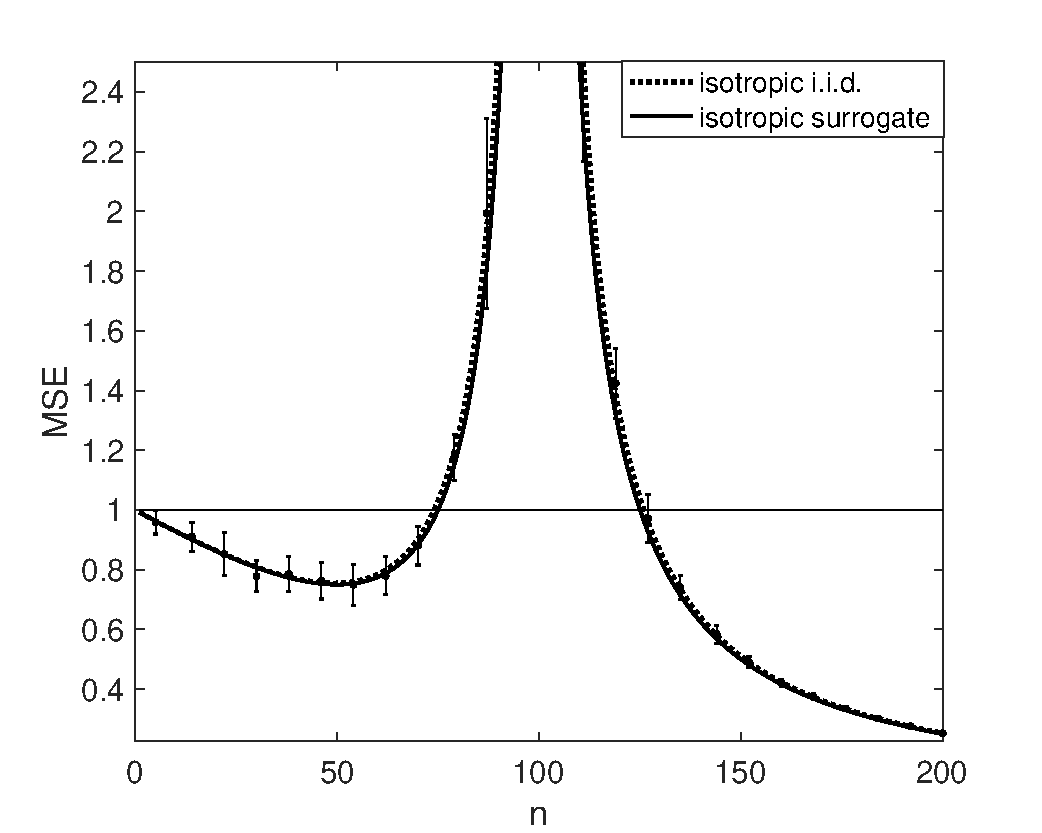
\includegraphics[width=0.7\textwidth]{../figs/descent-isotropic}
        \end{center}
\end{frame}

\begin{frame}
  \frametitle{Gaussian features: effect of spectral decay}
  $\X\sim\mu^n$ \ - multivariate Gaussian design,
  $\mu=\Nc(\zero,\Sigmab)$, $d=100$\\
$\Sigmab$ \ - exponentially decaying eigenvalues, condition
number $\kappa$
\pause
\begin{align*}
\MSE{\X^\dagger\y}\ =\ ?
  \end{align*}
  \pause \vspace{-3mm}
  \begin{center}
    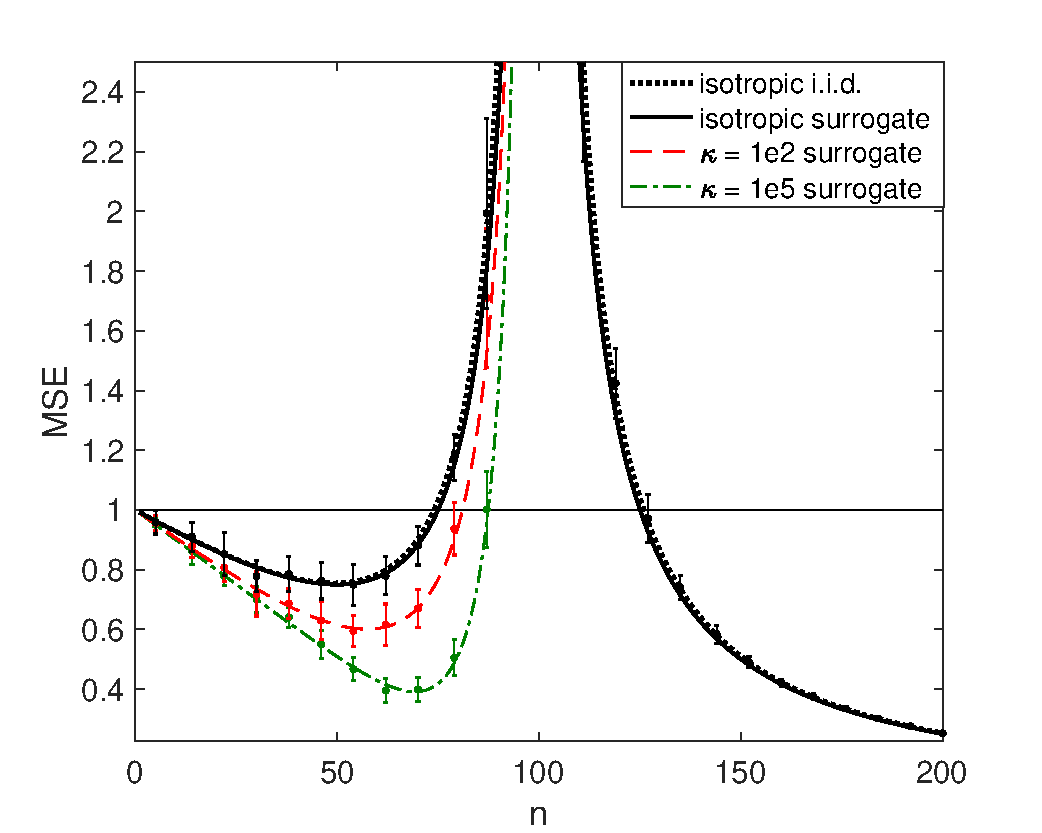
\includegraphics[width=0.7\textwidth]{../figs/descent-full}
  \end{center}
\end{frame}

\begin{frame}
  \frametitle{Gaussian features: effect of model complexity}
    $\X\sim\mu^n$ \ - multivariate Gaussian design,
  $\mu=\Nc(\zero,\Sigmab)$, $n=100$\\
$\Sigmab$ \ - exponentially decaying eigenvalues, condition
number $\kappa$
\begin{align*}
\MSE{\X^\dagger\y}\ =\ ?
  \end{align*}\vspace{-3mm}
  \begin{center}
    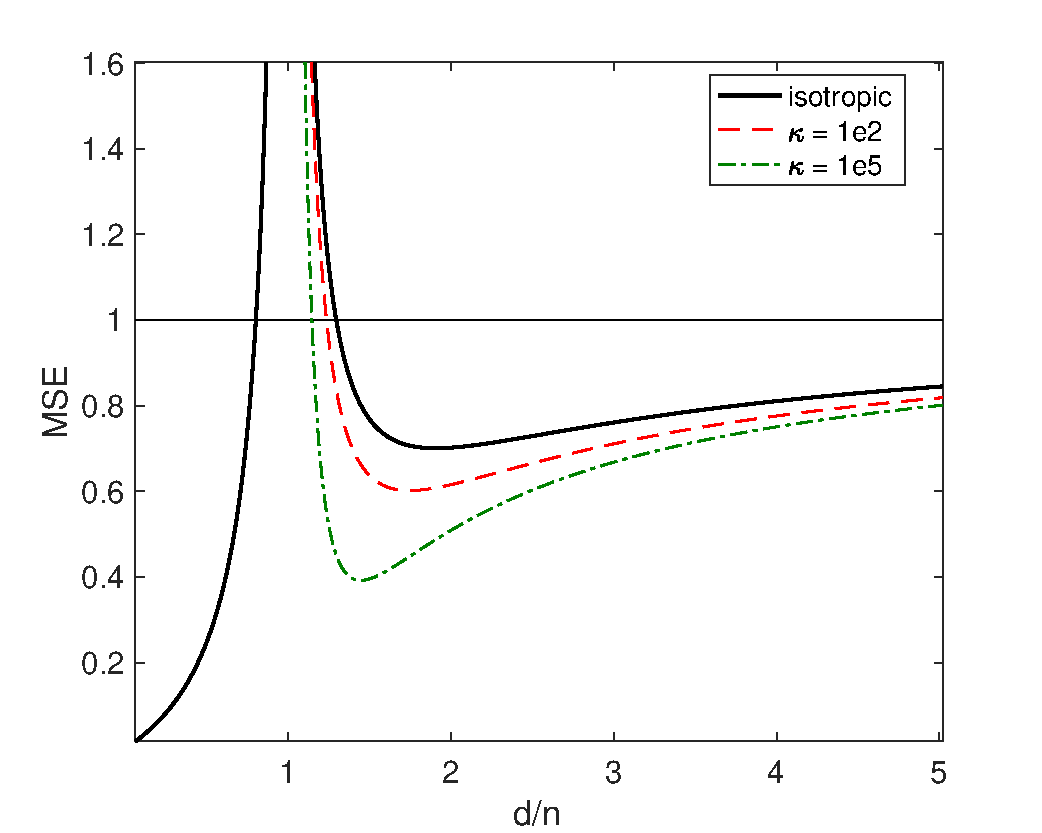
\includegraphics[width=0.7\textwidth]{../figs/descent-model}
  \end{center}
\end{frame}

\begin{frame}
  \frametitle{Main result II: implicit regularization of minimum norm}
Why does this \textit{unregularized} model learn when $n<d$?\\
  \pause
\textit{Because taking minimum norm induces
  $\ell_2$-regularization.}
\vspace{2mm}
\pause
\begin{theorem}
Let \ $\Xb\sim S_\mu^n$, \ $\yb_i=y(\x)$ \ and \
$\Sigmab_\mu=\E_\mu[\x\x^\top]$. Then,\pause
 \begin{align*}
    \E\big[\Xb^\dagger\ybb\big] = 
    \begin{cases}
       (\Sigmab_\mu + \lambda_n\I)^{-1}\v_{\mu,y} &\text{for }n<d,\\
        \Sigmab_\mu^{-1}\v_{\mu,y} &\text{for }n \ge d,
    \end{cases}
 \end{align*}
   where \ $n=\tr((\Sigmab_\mu+\lambda_n\I)^{-1}\Sigmab_\mu)$ \ and \ $\v_{\mu,y}=\E_\mu[y(\x)\,\x ]$.
\end{theorem}
\pause
\begin{align*}
  (\Sigmab_\mu +  \lambda_n\I)^{-1}\v_{\mu,y}
  \ =\ \argmin_{\wbh} \ \E_{\mu,y}\Big[\big(\x^\top\wbh-y(\x)\big)^2\Big]
    + \lambda_n\|\wbh\|^2
\end{align*}
\end{frame}

\begin{frame}
  \frametitle{Implicit regularization}
  Our observations:\\
  \begin{itemize}
    \item Minimum norm induces an $\ell_2$-regularizer:
      $\lambda_n\|\wbh\|^2$\pause
\item Sample size is effective dimension:
  $n=\tr((\Sigmab_\mu+\lambda_n\I)^{-1}\Sigmab_\mu)$
  \end{itemize}\pause
%\vspace{5mm}

~\hspace{-0.8cm}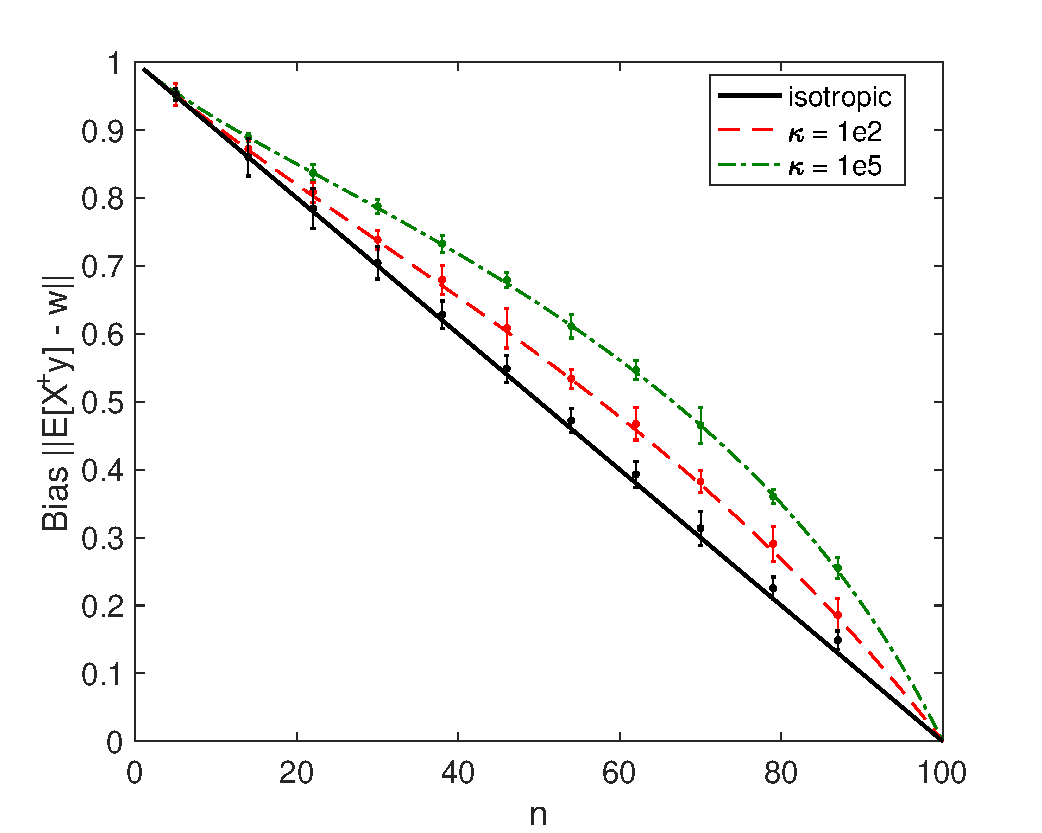
\includegraphics[width=0.57\textwidth]{../figs/descent-bias}\nobreak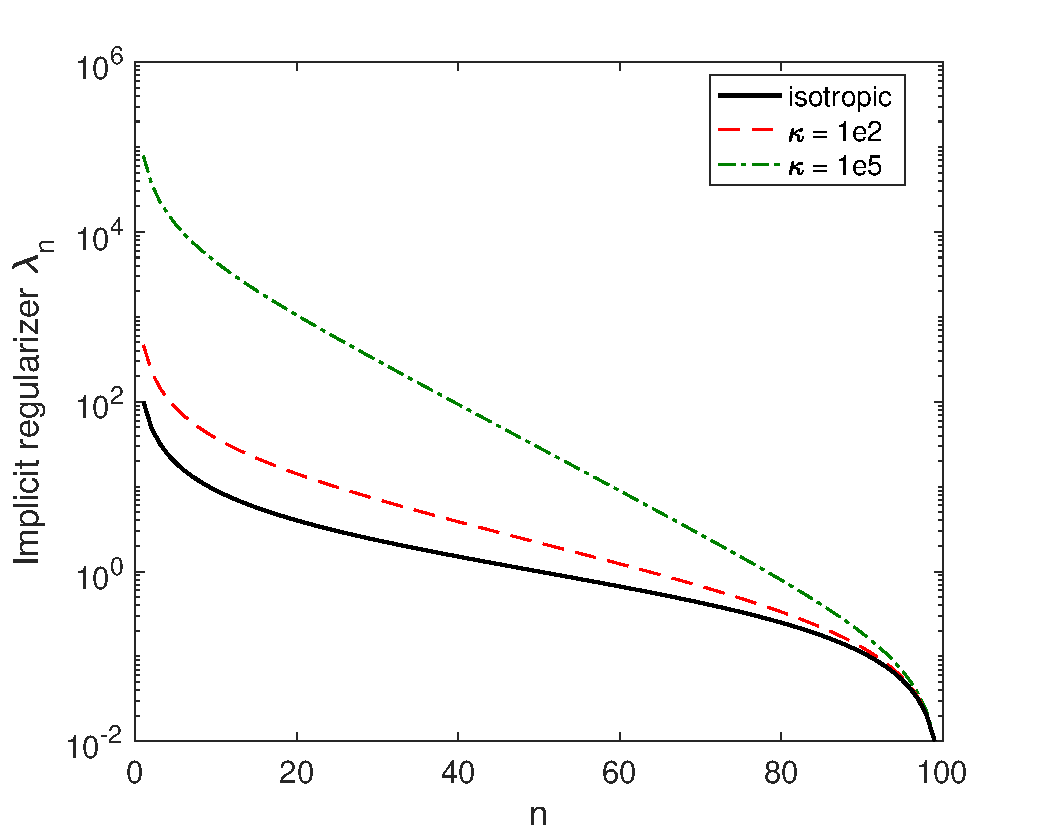
\includegraphics[width=0.57\textwidth]{../figs/descent-lambda}
\end{frame}

\begin{frame}
  \frametitle{Consistency of surrogate expressions}
  \begin{align*}
  \MSE{\X^\dagger\y}
  &=\sigma^2\E\big[\tr\big((\X^\top\X)^\dagger\big)\big] +
    \w^{\top}\E\big[\I-\X^\dagger\X\big]\w.
  \end{align*}
  \pause
  \begin{align*}
    \mu=\Nc(\zero,\Sigmab)\quad \Longrightarrow\quad
    \begin{cases}
      \X^\top\X&-\quad\text{Wishart distribution}\\
      \X^\dagger\X&-\quad\text{Gaussian projection}
    \end{cases}
  \end{align*}
  \pause
  \begin{conjecture}
  Fix $n/d<1$ and let $\mu=\Nc(\zero,\Sigmab )$, where 
  $c\I\preceq\Sigmab\preceq C\I$. Then:\pause
\begin{align*}
\bigg|\frac{\E\big[\tr((\X^\top\X)^\dagger)\big]}{\Vc(\Sigmab,n)} -1\bigg|&=
  O(1/d)\quad\text{for}\quad\Vc(\Sigmab,n)=\frac{1-\alpha_n}{\lambda_n},\\
\onslide<5>{  %\sup_{\w\in\R^d}
  \bigg|\frac{\w^\top\E[\I-\X^\dagger\X]\w}{\w^\top
  \Bc(\Sigmab,n)\w} - 1\bigg| &= O(1/d)\quad\text{for}\quad
  \Bc(\Sigmab,n) = \lambda_n(\Sigmab+\lambda_n\I)^{-1}.}
\end{align*}
\end{conjecture}
\end{frame}

\begin{frame}
  \frametitle{Empirical evidence for the conjecture}
~\hspace{-1cm}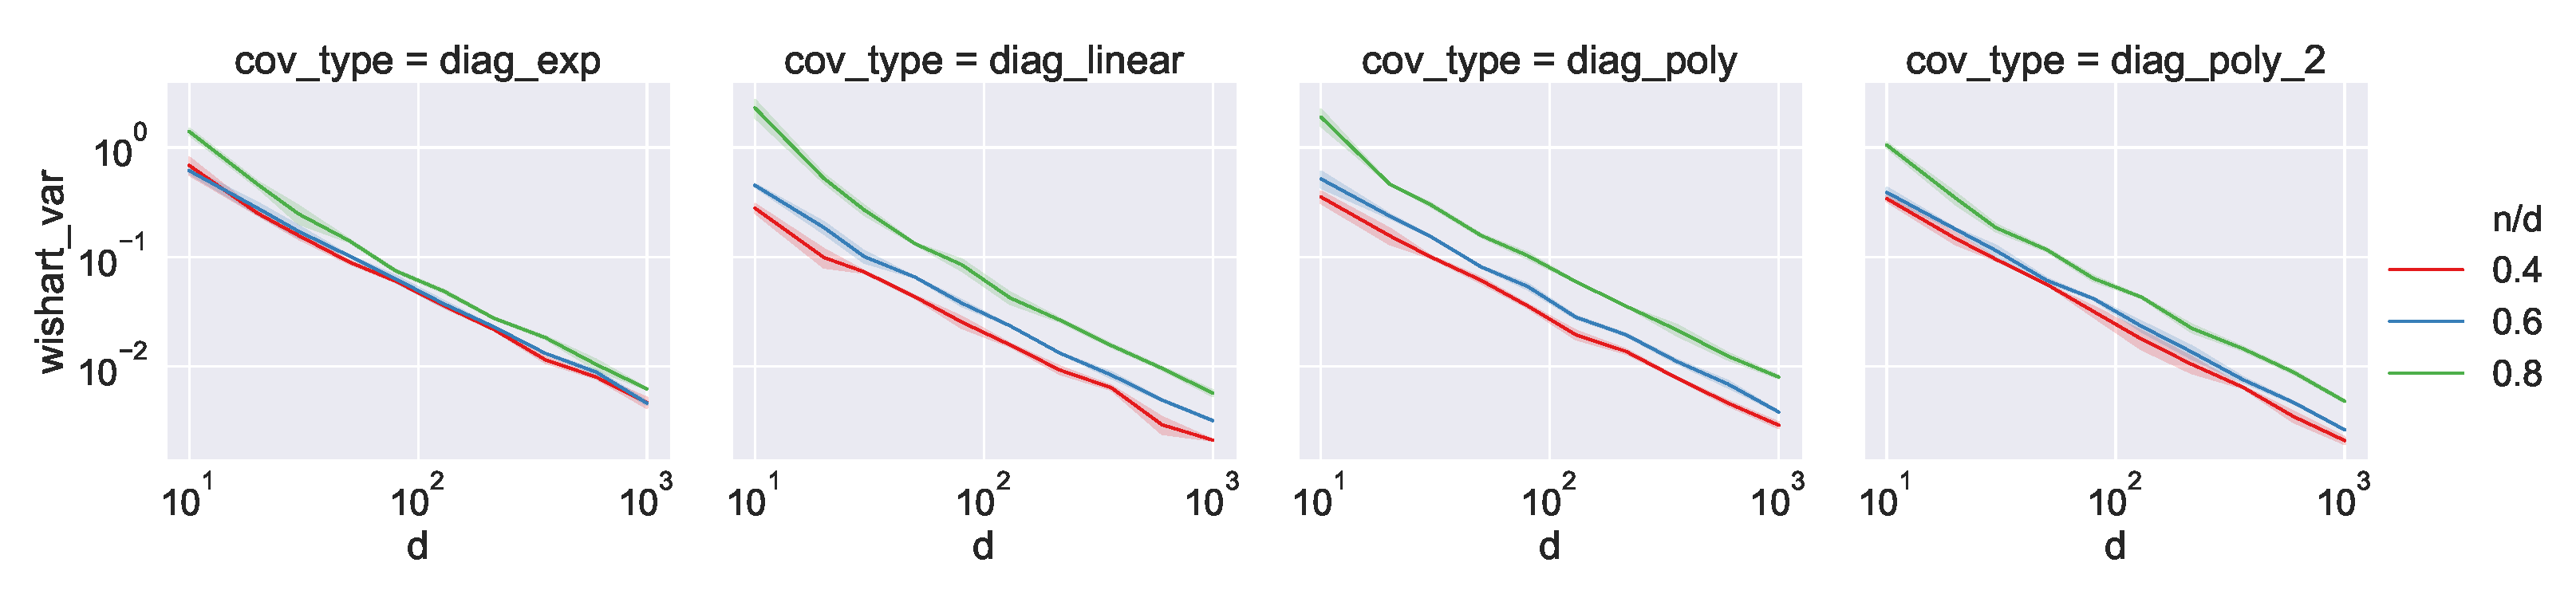
\includegraphics[width=1.16\textwidth]{../continuous_figures/wishart_var.pdf}\\
~\hspace{-1cm}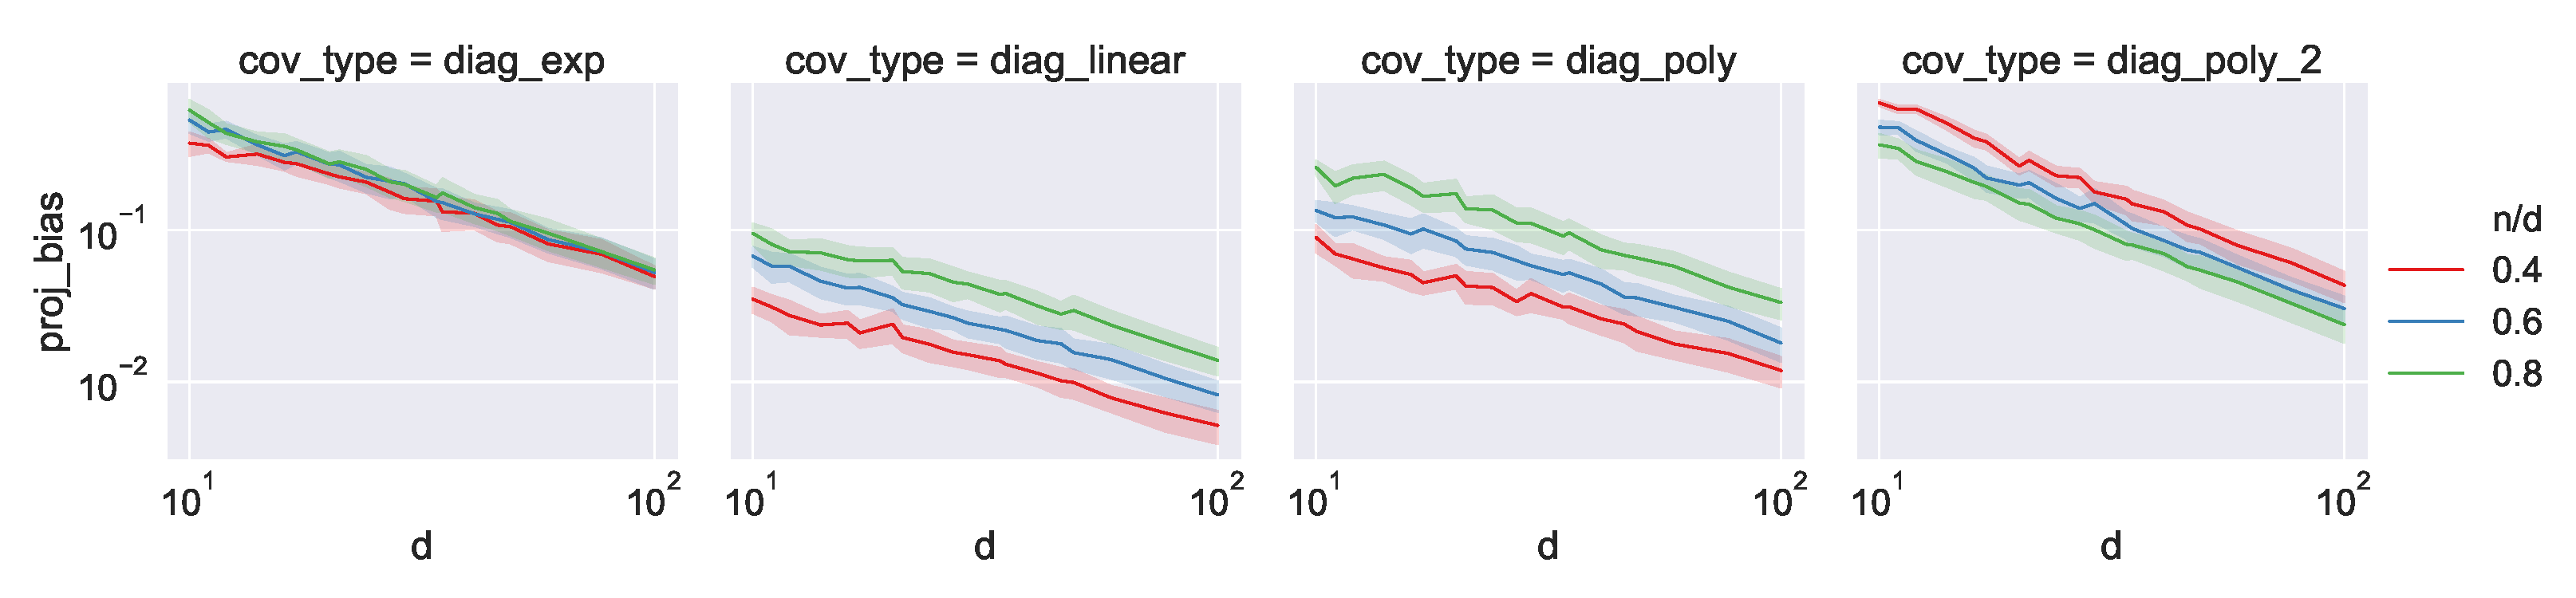
\includegraphics[width=1.16\textwidth]{../continuous_figures/proj_bias.pdf}
\end{frame}

\begin{frame}
  \frametitle{Surrogate design: rescaling by pseudo-determinant}
  \begin{definition}
    Let $K$ be a random variable over non-negative integers. \\
    A determinantal surrogate design
    $\Xb\sim \Det(\mu,K)$ is defined so that
\begin{align*}
  \E\big[F(\Xb)\big]\  \propto\ \E[\pdet(\X\X^\top)F(\X)]
  \quad\text{for}\quad\X\sim\mu^K.
\end{align*}
\end{definition}
\begin{itemize}
  \pause
\item The proportionality constant is $1/\E[\pdet(\X\X^\top)]$.
\pause
\item To compute it, we let $K$ be a Poisson random variable.
\pause
\item New expectation formulas for $K\sim\Poisson(\gamma)$ and $\X\sim\mu^K$:
\begin{align*}
  \E\big[\det(\X\X^\top)\big]
  &= \ee^{-\gamma}\det(\I+\gamma\Sigmab_\mu)\\
  \E\big[\det(\X^\top\X)\big]
  &= \det(\gamma\Sigmab_\mu)
\end{align*}
\end{itemize}

\end{frame}

\begin{frame}
  \frametitle{New technique: \textit{determinant preserving random
      matrices}}
\begin{definition}
A random $d\times d$ matrix $\A$ is \emph{determinant
  preserving} (d.p.) if
\begin{align*}
  \E\big[\!\det(\A_{\Ic,\Jc})\big] =
  \det\!\big(\E[\A_{\Ic,\Jc}]\big)\quad \text{for all }\Ic,\Jc\subseteq
  [d]\text{ s.t. }|\Ic|=|\Jc|.
\end{align*}
\vspace{-7mm}
\end{definition}
\pause
Examples:
  \begin{itemize}
  \item $\A$ has i.i.d.~Gaussian entries  $a_{ij}\sim\Nc(0,1)$\pause    
  \item $\A = s\Z$, where $s$ is random and $\Z$ is a fixed,
    rank-1 matrix\pause
    \item $\A=\X^\top\X$, where $\X\sim\mu^K$ and $K\sim\Poisson(\gamma)$
    \end{itemize}
    \pause
  \begin{theorem}[closure properties]
    If $\A,\B$ are d.p.~and independent, then $\A+\B$ and $\A\B$ are
    also d.p.
  \end{theorem}
\end{frame}

\begin{frame}
  \frametitle{Next steps}
  \begin{itemize}
  \item Consistency of surrogate expressions\\[3mm]\pause
  \item Random feature models\\[3mm]\pause
  \item Non-linear and kernelized models\\[3mm]\pause
  \item Prediction error
  \end{itemize}
\end{frame}

\begin{frame}
  \frametitle{References}
  \footnotesize
\bibliographystyle{alpha}
\bibliography{../pap}
\end{frame}

\end{document}